\paragraph{Tiled Matrix Multiplication}

In the following section, we present an \textbf{example of matrix multiplication using the tiling technique} to illustrate the efficiency improvements brought about by the tiling technique.

\highspace
\begin{flushleft}
    \textcolor{Green3}{\faIcon{book} \textbf{Traditional approach}}
\end{flushleft}
Classical matrix multiplication has the following characteristics
\begin{itemize}
    \item Each thread accesses a row of matrix $M$ and a column of matrix $N$.
    \item Each thread block accesses a strip of matrix $M$ and a strip of matrix $N$.
\end{itemize}
\begin{figure}[!htp]
    \centering
    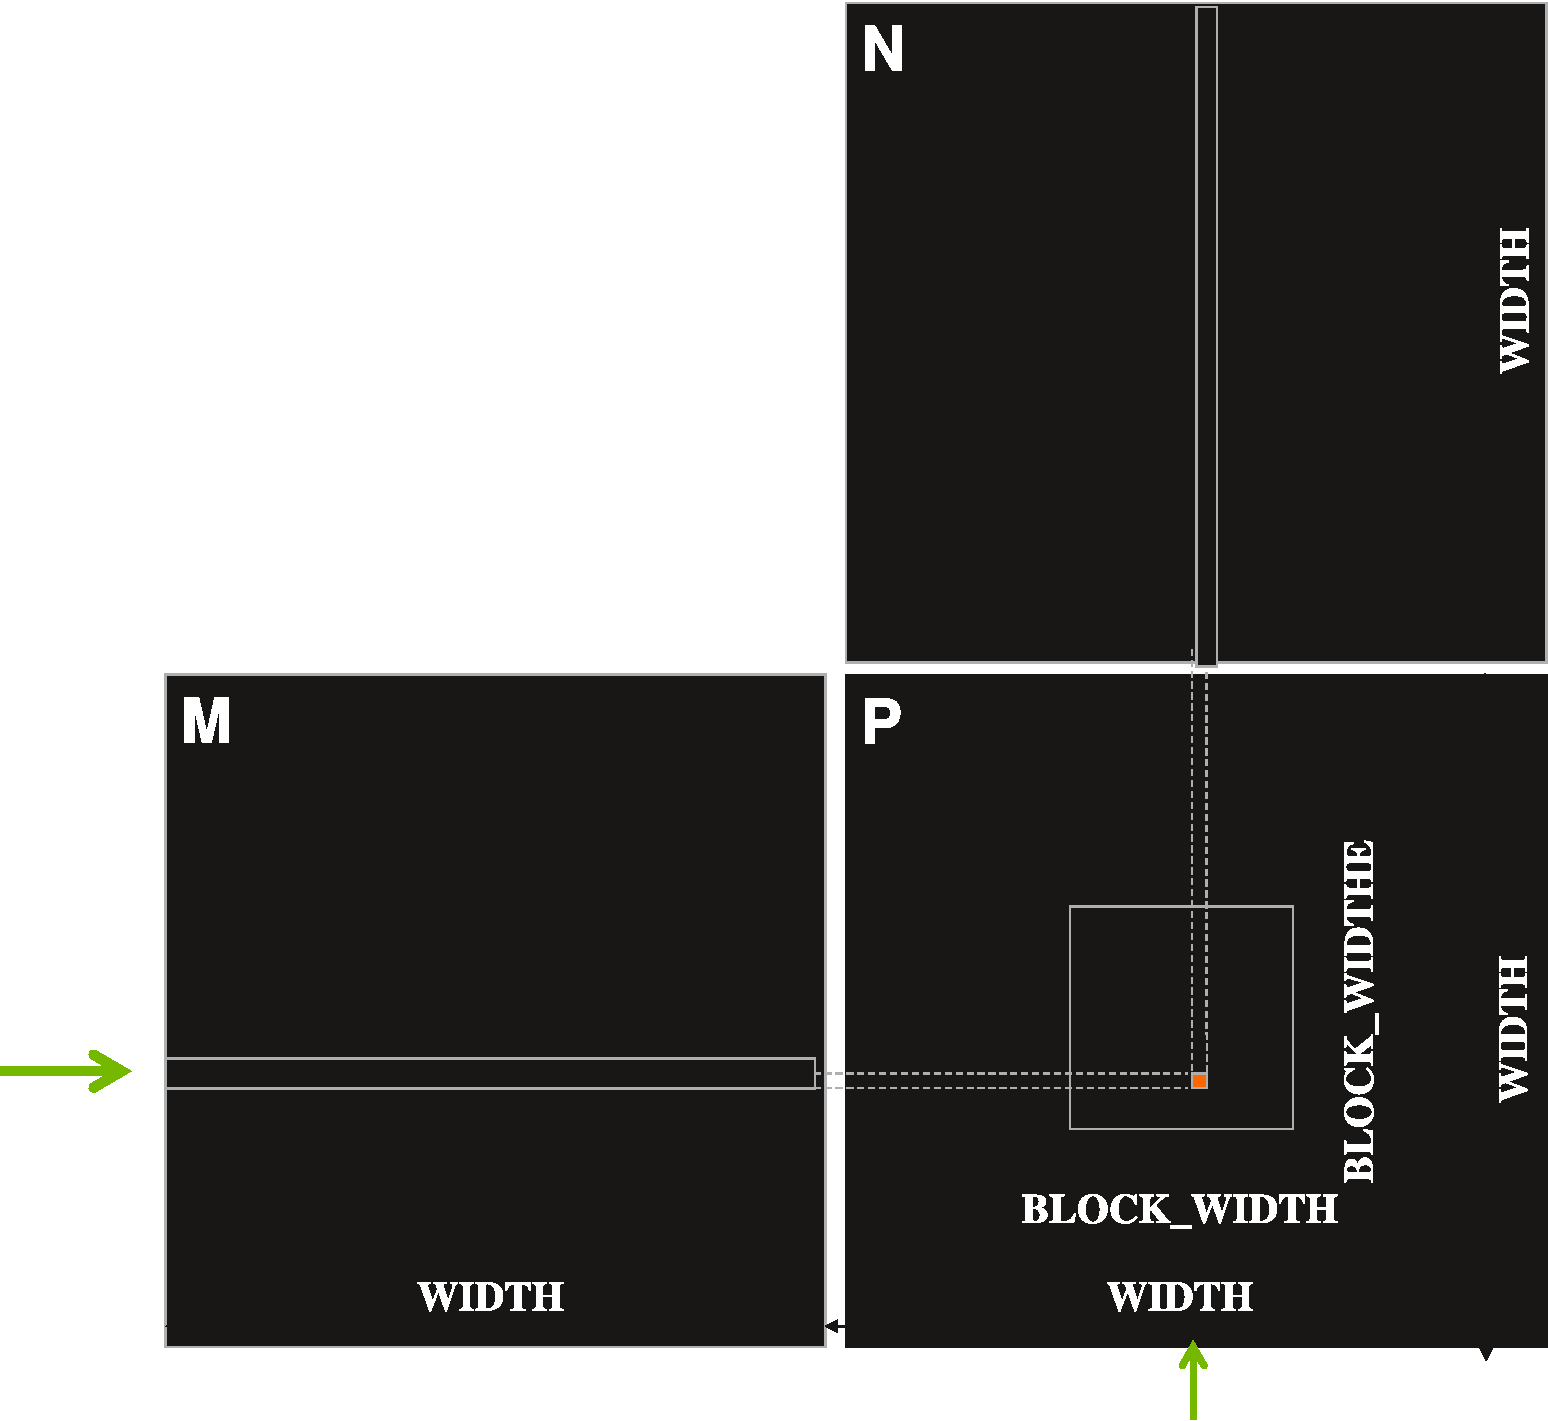
\includegraphics[width=.8\textwidth]{img/cuda-matrix-multiplication-1.pdf}
\end{figure}
In the traditional approach, threads access data directly from global memory, which can be inefficient due to high latency.

\begin{flushleft}
    \textcolor{Green3}{\faIcon{tachometer-alt} \textbf{Tiled Matrix Multiplication}}
\end{flushleft}
\begin{enumerate}
    \item As a \textbf{first step}, since we know the problem and (ideally) how the solution is implemented, we can try to brainstorm on how to apply tiling. In general, matrix operations lend themselves well to the tiling technique. In the matrix multiplication:
    \begin{itemize}
        \item The execution of each thread can be broken into phases.
        \item The data accesses by the thread block in each phase are focused on one tile of $M$ and one tile of $N$.
        \item The tile is of \texttt{BLOCK\_SIZE} elements in each dimension.
    \end{itemize}


    \item As second step, the threads in a block participate in \textbf{loading items into shared memory using the tiling technique}.
    
    As we can see in the following figure, each thread in a block contributes to loading elements from matrices $M$ and $N$ into shared memory. Each thread is responsible for loading one element from the $M$ matrix and one element from the $N$ matrix into shared memory. This parallel loading ensures that data is moved quickly and efficiently from global memory to faster shared memory.

    \begin{figure}[!htp]
        \centering
        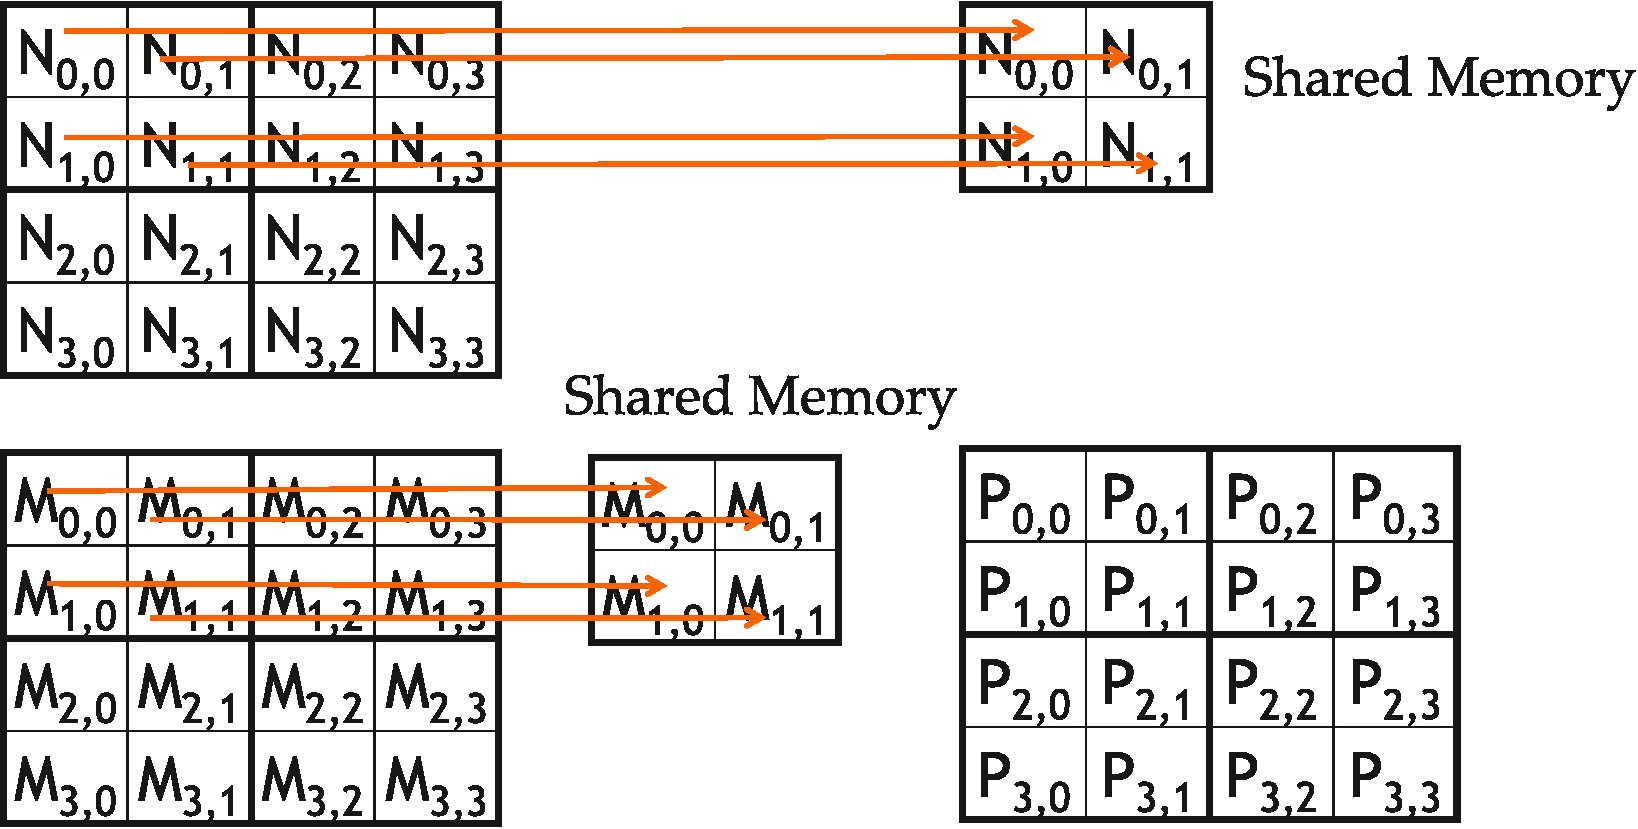
\includegraphics[width=.8\textwidth]{img/cuda-tiled-matrix-multiplication-1.pdf}
    \end{figure}

    The matrices $M$ and $N$ are the input and $P$ is the result matrix. Each element is indexed by $i$ and $j$ (e.g., $M_{ij}$).
    \begin{itemize}
        \item Elements of $M$ are loaded into shared memory by the threads.
        \item Similarly, elements of $N$ are loaded into shared memory.
    \end{itemize}
    This particular phase focuses on the initial loading of elements for the tile corresponding to block (0,0). Each thread in block (0,0) loads one element from $M$ and one from $N$, populating the shared memory with the necessary data for the computation.

    These steps are performed for each block of the matrices. In the following figure, we can see another step of loading into shared memory.
    \begin{figure}[!htp]
        \centering
        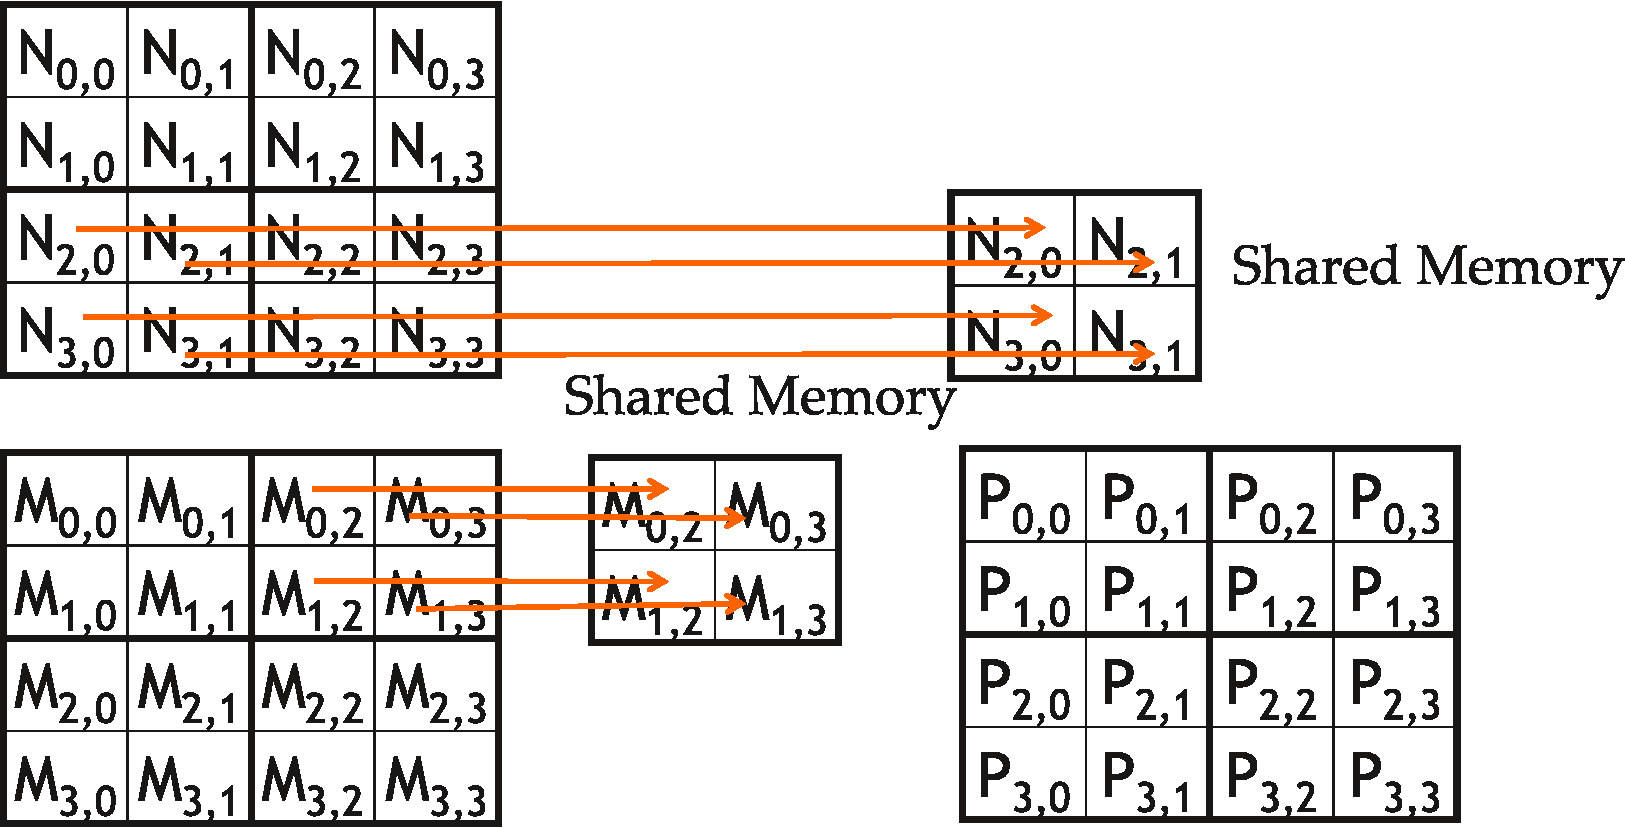
\includegraphics[width=.8\textwidth]{img/cuda-tiled-matrix-multiplication-4.pdf}
    \end{figure}


    \newpage
    \item After loading into shared memory, there is the loading step, done in two iterations, into the result matrix. This is only a graphical representation, because in reality this step can be merged with the execution step. This step prepares the operands to be used in the execution step.
    \begin{enumerate}
        \item In the first iteration, the elements from the shared memory $N_{0,0}, N_{0,1}$ are used against the element from the shared memory $M_{0,0}, M_{1,0}$.
        \begin{figure}[!htp]
            \centering
            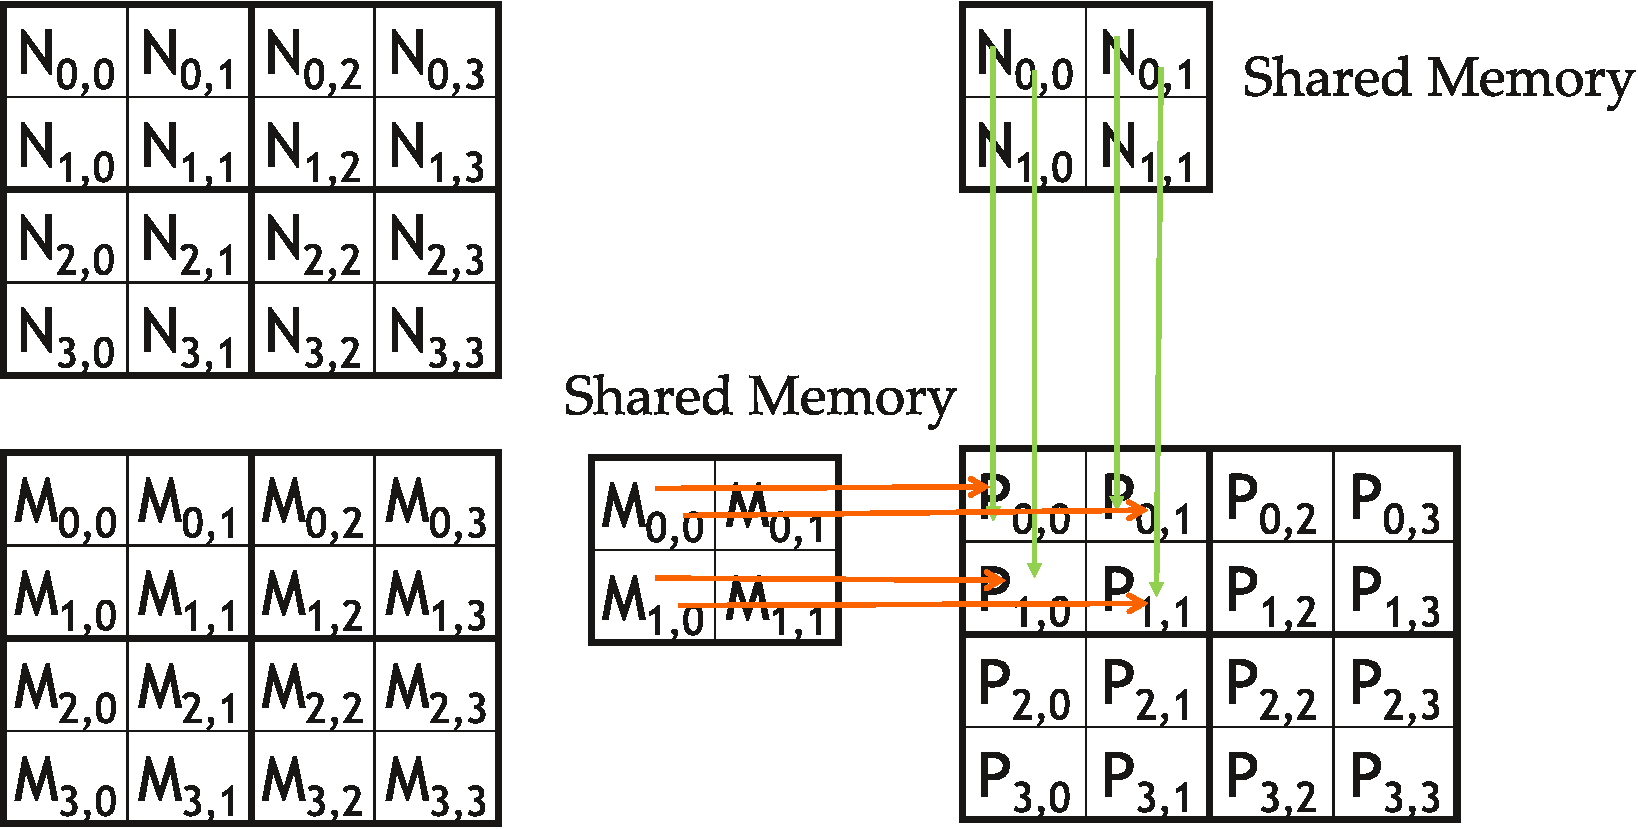
\includegraphics[width=.8\textwidth]{img/cuda-tiled-matrix-multiplication-2.pdf}
        \end{figure}
        \item In the second iteration, the elements from the shared memory $N_{1,0}, N_{1,1}$ are used against the element from the shared memory $M_{0,1}, M_{1,1}$.
        \begin{figure}[!htp]
            \centering
            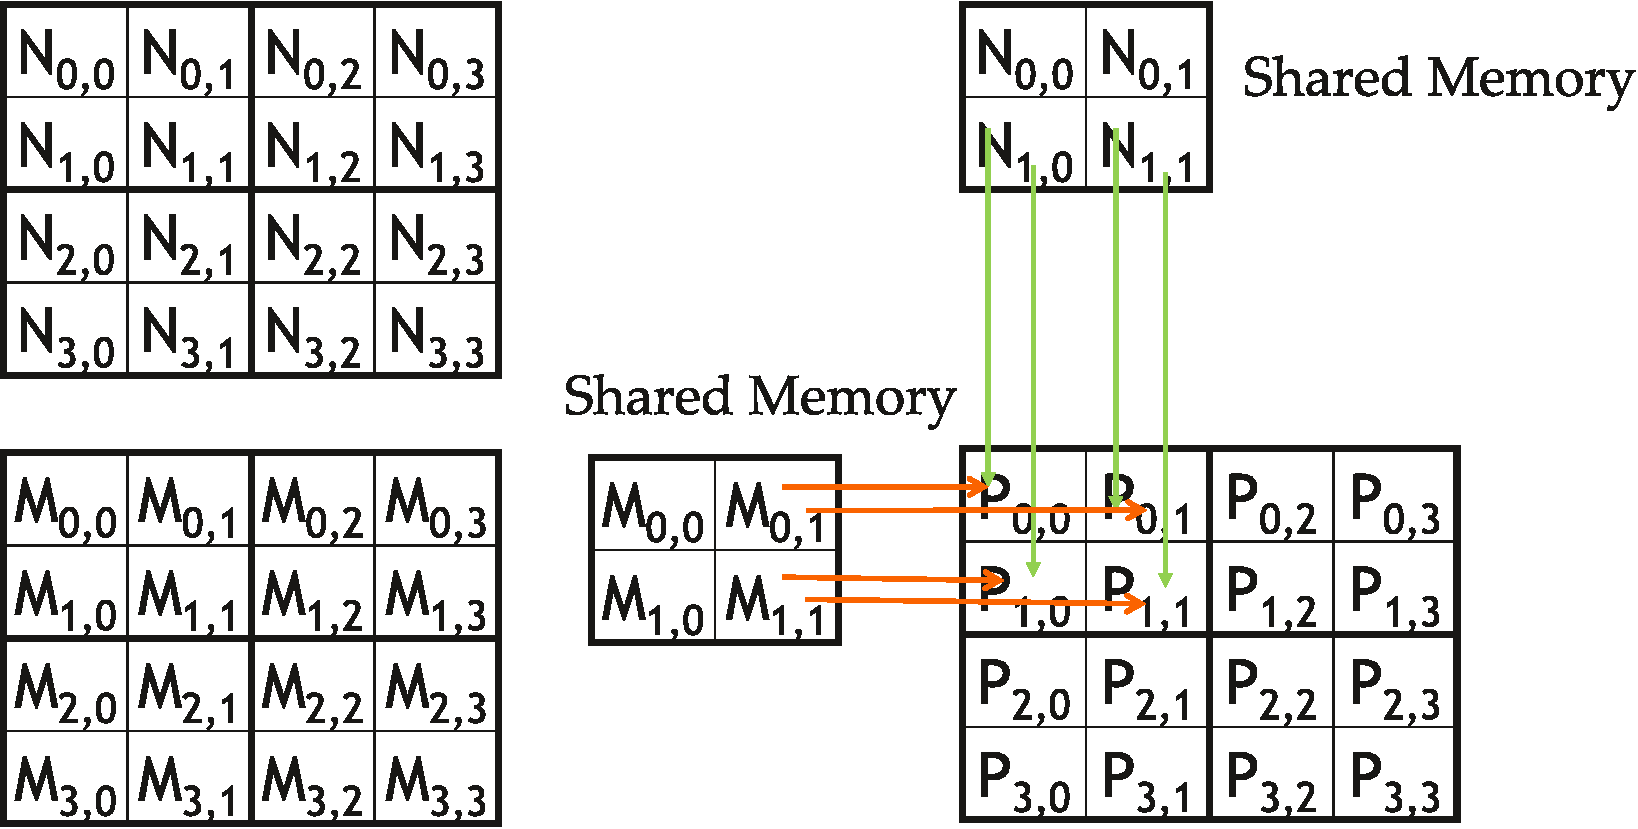
\includegraphics[width=.8\textwidth]{img/cuda-tiled-matrix-multiplication-3.pdf}
        \end{figure}
    \end{enumerate}
    This step is done for each block of the matrices. In the figure on the next page, we can see two more steps of the load block.
    \newpage
    \begin{figure}[!htp]
        \centering
        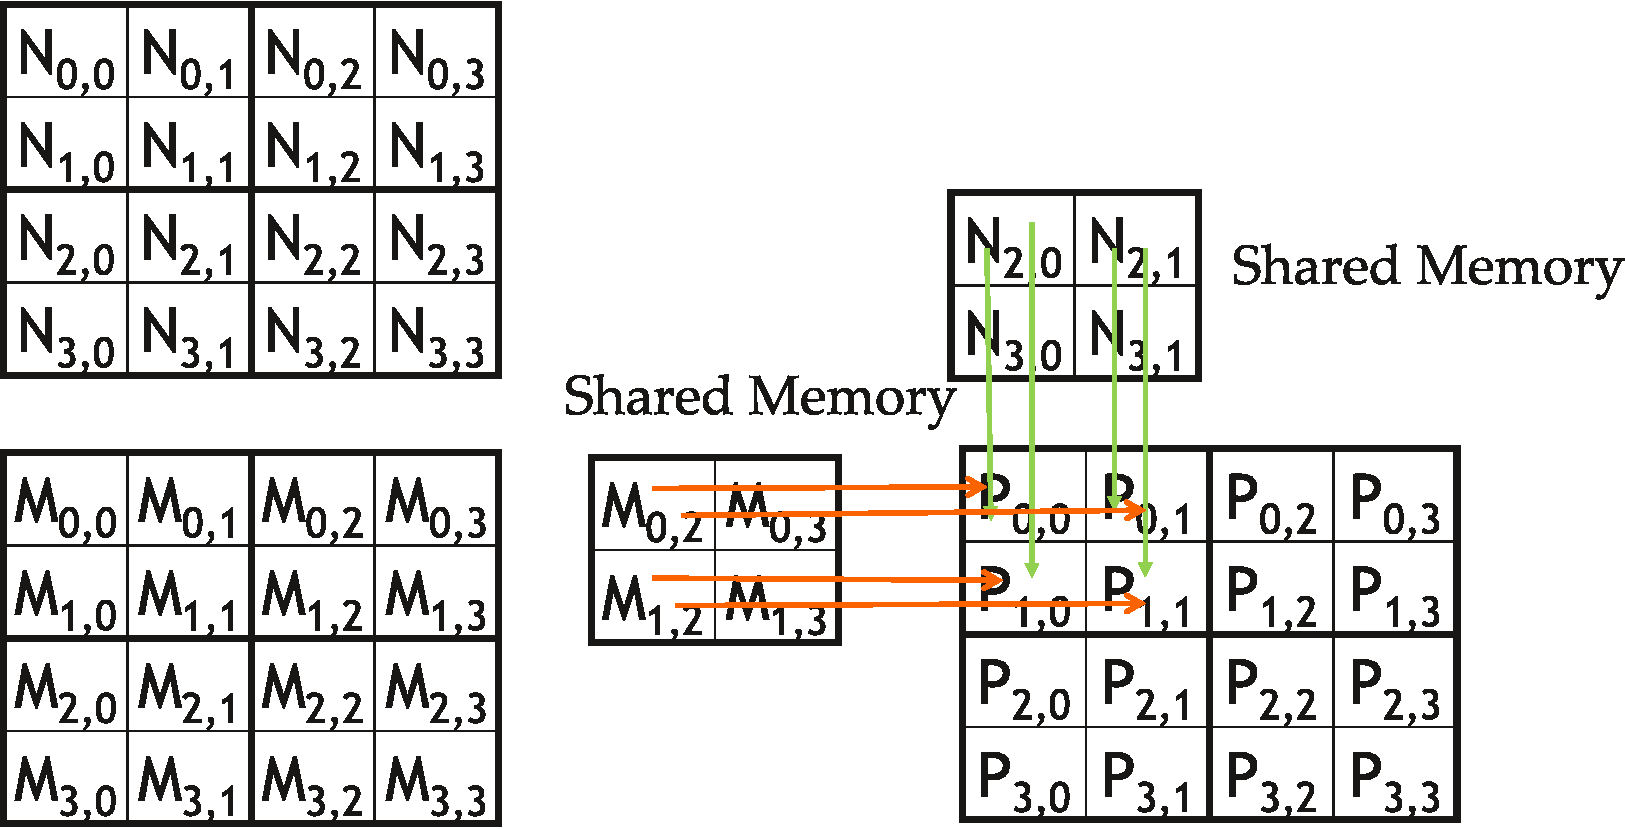
\includegraphics[width=.8\textwidth]{img/cuda-tiled-matrix-multiplication-5.pdf}
    \end{figure}
    \begin{figure}[!htp]
        \centering
        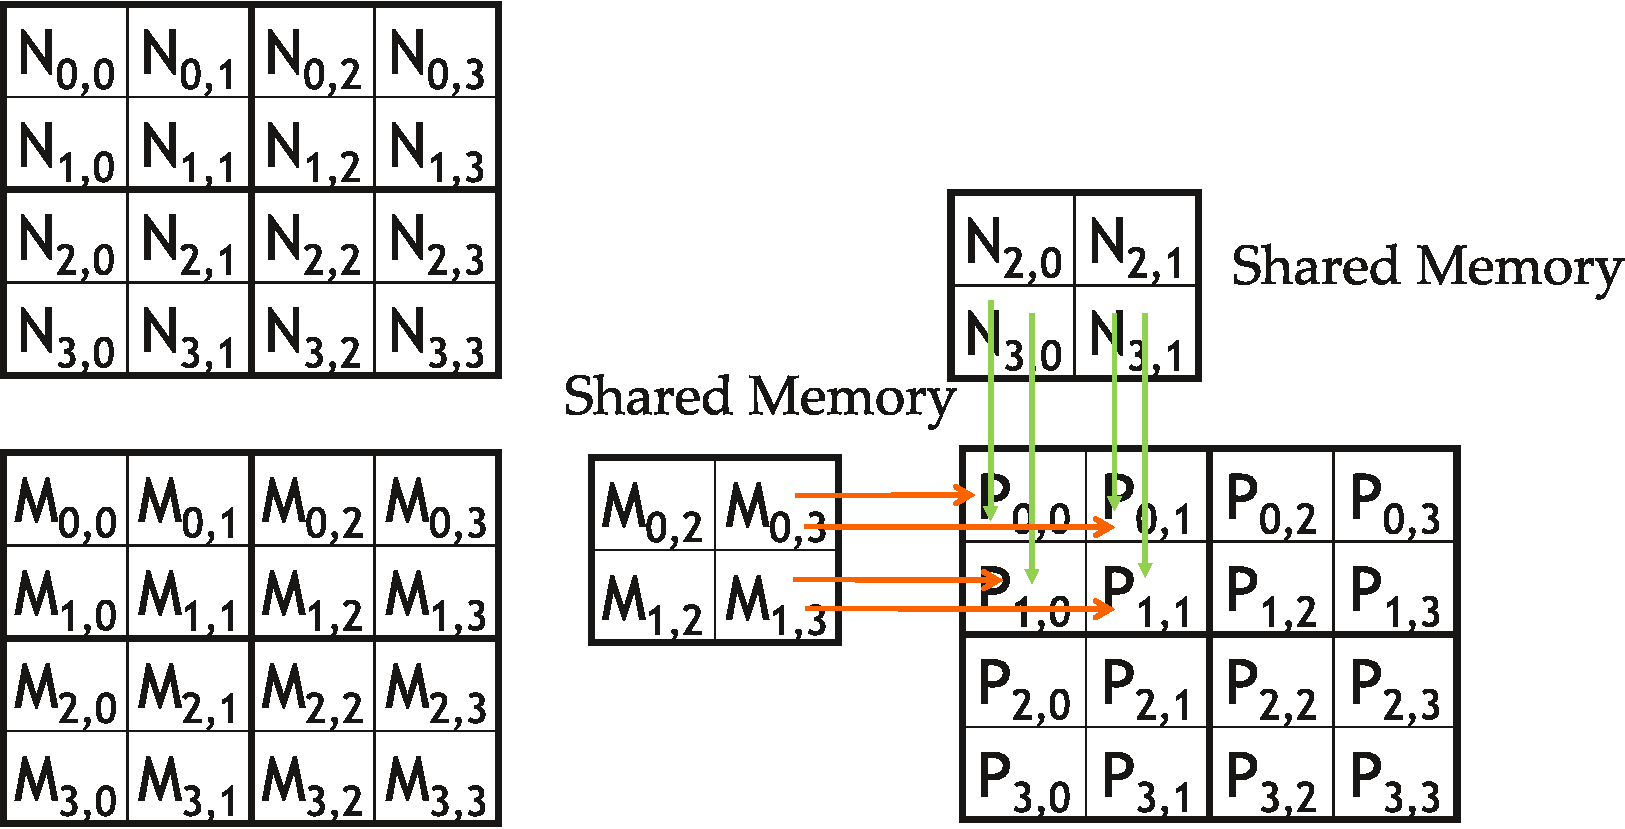
\includegraphics[width=.8\textwidth]{img/cuda-tiled-matrix-multiplication-6.pdf}
    \end{figure}


    \item After each load, there is the \textbf{execution phase}. In the following table, we highlight how four threads in a block perform matrix multiplication using shared memory.
    \begin{figure}[!htp]
        \centering
        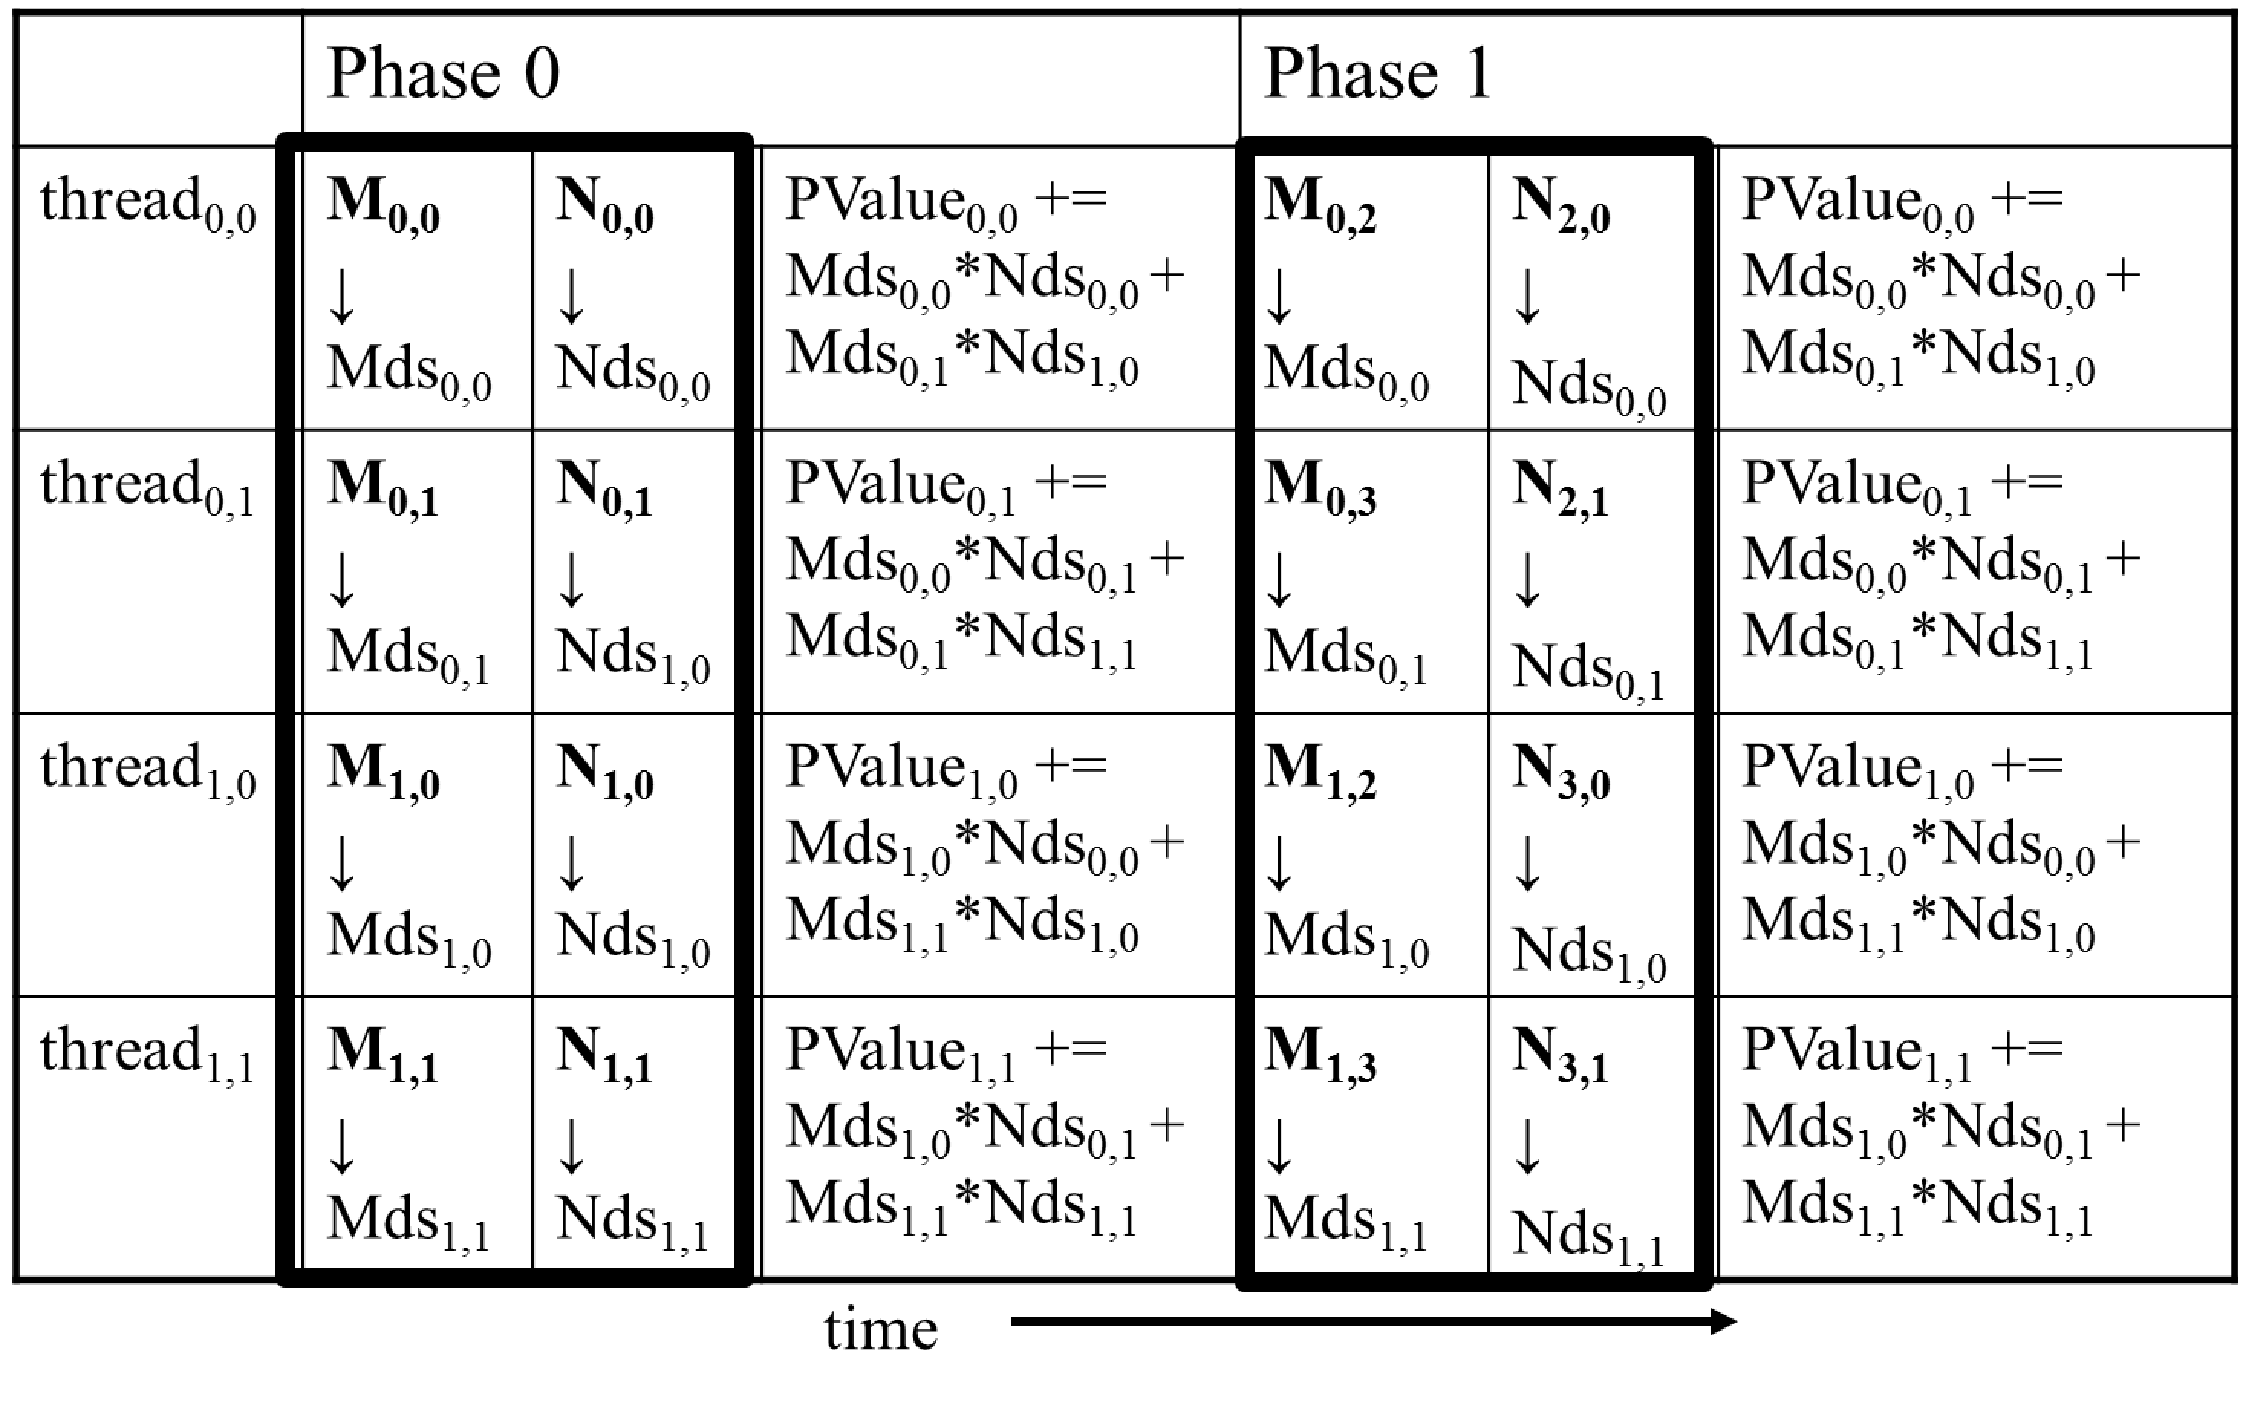
\includegraphics[width=\textwidth]{img/cuda-tiled-matrix-multiplication-7.pdf}
    \end{figure}
    \newpage
    The values $\texttt{Mds}_{i,j}$ are the values loaded in the load step from global to shared memory of the $M$ matrix. The same reasoning applies to $\texttt{Nds}$.

    Once the data is loaded into shared memory, each thread uses the loaded values to update the partial product value $\texttt{PValue}$ for the resulting matrix $P$:
    \begin{itemize}
        \item $\texttt{thread}_{0,0}$:
        \begin{lstlisting}[language=C++]
$\texttt{PValue}_{0,0}$ += $\texttt{Mds}_{0,0}$ * $\texttt{Nds}_{0,0}$ + $\texttt{Mds}_{0,1}$ * $\texttt{Nds}_{1,0}$\end{lstlisting}

        \item $\texttt{thread}_{0,1}$:
        \begin{lstlisting}[language=C++]
$\texttt{PValue}_{0,1}$ += $\texttt{Mds}_{0,0}$ * $\texttt{Nds}_{0,1}$ + $\texttt{Mds}_{0,1}$ * $\texttt{Nds}_{1,1}$\end{lstlisting}
        \item $\texttt{thread}_{1,0}$:
        \begin{lstlisting}[language=C++]
$\texttt{PValue}_{1,0}$ += $\texttt{Mds}_{1,0}$ * $\texttt{Nds}_{0,0}$ + $\texttt{Mds}_{1,1}$ * $\texttt{Nds}_{1,0}$\end{lstlisting}
        \item $\texttt{thread}_{1,1}$:
        \begin{lstlisting}[language=C++]
$\texttt{PValue}_{1,1}$ += $\texttt{Mds}_{1,0}$ * $\texttt{Nds}_{0,1}$ + $\texttt{Mds}_{1,1}$ * $\texttt{Nds}_{1,1}$\end{lstlisting}
    \end{itemize}

    \item \textbf{Barrier Synchronization step}. To synchronize all threads in a block, we use the function \texttt{\_\_syncthreads()}. This function acts as a barrier synchronization, ensuring that all threads in a block reach that point before any thread can proceed.
    
    Barrier synchronization is particularly useful for coordinating the execution of tiled algorithms in phases. It is useful in:
    \begin{itemize}[label=\textcolor{Green3}{\faIcon{check}}]
        \item \textbf{Loading Phase}. Ensures that \textbf{all elements of a tile are loaded into shared memory before any computation begins}.
        \item \textbf{Computation Phase}. Ensures that \textbf{all threads have completed their computation on the current tile before moving to the next phase or tile}.
    \end{itemize}
\end{enumerate}
